
\documentclass[black]{beamer}
\usetheme{Warsaw}

\usefonttheme{serif}


\definecolor{CUorange}{RGB}{246, 103, 51}
\definecolor{CUpurple}{RGB}{82, 45, 128}

\setbeamercolor*{palette primary}{use=structure,fg=white,bg=CUorange}
\setbeamercolor*{palette quaternary}{fg=white,bg=CUpurple}

\newcommand*\Myitem{% 
    \item[\color{CUpurple}{\ding{111}}]}
    
%\newcommand*\Myitem1{% 
%    \item[\color{CUpurple}{1.}]}
%\newcommand*\Myitem2{% 
%    \item[\color{CUpurple}{2.}]}
%\newcommand*\Myitem3{% 
%    \item[\color{CUpurple}{3(i).}]}
%\newcommand*\Myitem4{% 
%    \item[\color{CUpurple}{3(ii).}]}    


\usepackage{color, caption, bm}
\usepackage[english]{babel}
\usepackage[latin1]{inputenc}
%\usepackage{times}
\usepackage{pifont}
\usepackage[T1]{fontenc}
\usepackage{graphicx}
\usepackage{subfigure}
\usepackage{color}
\usepackage{amsmath}
\usepackage[latin1]{inputenc}
\usepackage{tikz}
\usetikzlibrary{shapes,arrows}

\newcommand{\mb}[1]{\mathbf{#1}}       % bold letters in mathmode
\newcommand{\bs}[1]{\boldsymbol{#1}}   % bold symbols in mathmode



\title{A clever proposal distribution for Metroplis-Hastings}
%\subtitle{ If a subtitle is needed}
\author{Chase Joyner}
\institute{MATH 802}
\date



\begin{document}

\begin{frame}
  \titlepage
\end{frame}

\begin{frame}
\frametitle{Outline}
\begin{itemize}
\item Motivate and introduce Bayesian Statistics
\vspace{0.2cm}
\item Metropolis--Hastings
\vspace{0.2cm}
\item Generalized Linear Models (brief)
\vspace{0.2cm}
\item Bayesian Iteratively Weighted Least Squares (BIWLS)
\vspace{0.2cm}
\item Discussion of BIWLS
\vspace{0.2cm}
\item Small example
\end{itemize}
\end{frame}

\begin{frame}
\frametitle{Motivation}
\begin{itemize}
\item Suppose you flip a fair coin 100 times and recorded 64 heads and 36 tails.
\vspace{0.2cm}
\item The sample percentage of heads is 0.64, but $P(\text{heads}) = 0.5$.
\vspace{0.2cm}
\item {\it A priori} of flipping the coin, we believe it to be fair.  We can use this.
\vspace{0.2cm}
\item Looking for your phone.
\vspace{0.2cm}
\item Nate Silver used Bayesian statistics to
\vspace{0.2cm}
\begin{itemize}
\Myitem predict the results of the 2008 presidential election and got 49 out of the 50 states correct.
\vspace{0.1cm}
\Myitem predict the results of the 2012 presidential election and got 50 out of the 50 states correct.
\end{itemize}
\end{itemize}
\end{frame}

\begin{frame}
\frametitle{Bayesian Inference}
Bayesian inference uses Bayes rule to obtain a posterior distribution.
\begin{center}
\begin{itemize}
\item {\it A priori} information specified through a prior distribution, denoted $\pi(\boldsymbol\theta)$.
\item Likelihood function, denoted $f({\bf y}|\boldsymbol\theta)$, specified by the data.
\end{itemize}
\[
f(\boldsymbol\theta|{\bf y}) = \frac{f({\bf y}| \boldsymbol\theta)\pi(\boldsymbol\theta)}{f({\bf y})} = \frac{f({\bf y}| \boldsymbol\theta)\pi(\boldsymbol\theta)}{\int_\Theta f({\bf y}|\boldsymbol\theta)\pi(\boldsymbol\theta)d\boldsymbol\theta} \propto f({\bf y}| \boldsymbol\theta)\pi(\boldsymbol\theta)
\]
\end{center}
\begin{itemize}
\item $f(\boldsymbol\theta|{\bf y})$ is the posterior distribution.  It is an update of $\pi(\boldsymbol\theta)$ after seeing ${\bf y}$.
\end{itemize}
\end{frame}

\begin{frame}
\frametitle{Metropolis--Hastings}
\begin{itemize}
\item The posterior distribution $f(\boldsymbol\theta|{\bf y})$ not of any known form.
\vspace{0.2cm}
\item Want to obtain a sequence of samples $\{\boldsymbol\theta^{(1)},...,\boldsymbol\theta^{(s)}\}$ to empirically estimate $\bm\theta$.
\vspace{0.2cm}
\item Intuitively, include new $\boldsymbol\theta^{\star}$ if its posterior density is greater than current $\boldsymbol\theta^{(t)}$, else accept it with probability $r$.
\vspace{0.2cm}
\begin{itemize}
\Myitem $r = \frac{f(\boldsymbol\theta^\star | {\bf y})}{f(\boldsymbol\theta^{(t)}|{\bf y})}\frac{J(\boldsymbol\theta^{(t)}|\boldsymbol\theta^\star)}{J(\boldsymbol\theta^\star|\boldsymbol\theta^{(t)})} = \frac{f({\bf y}|\boldsymbol\theta^\star)\pi(\boldsymbol\theta^\star)}{f({\bf y}|\boldsymbol\theta^{(t)})\pi(\boldsymbol\theta^{(t)})}\frac{J(\boldsymbol\theta^{(t)}|\boldsymbol\theta^\star)}{J(\boldsymbol\theta^\star|\boldsymbol\theta^{(t)})}$
\vspace{0.2cm}
\end{itemize}
\item Propose $\boldsymbol\theta^\star$ from some proposal distribution, denoted $J$.
\begin{itemize}
\Myitem Use this proposal distribution to calculate $\frac{J(\boldsymbol\theta^{(t)}|\boldsymbol\theta^\star)}{J(\boldsymbol\theta^\star|\boldsymbol\theta^{(t)})}$ in $r$ above.  This is the correction factor, in case $\boldsymbol\theta^\star$ is more likely to be proposed than $\boldsymbol\theta^{(t)}$.  Otherwise, $\boldsymbol\theta^\star$ will be over--represented in our sequence.
\end{itemize}
\end{itemize}
\end{frame}

\begin{frame}
\frametitle{Metropolis--Hastings cont.}
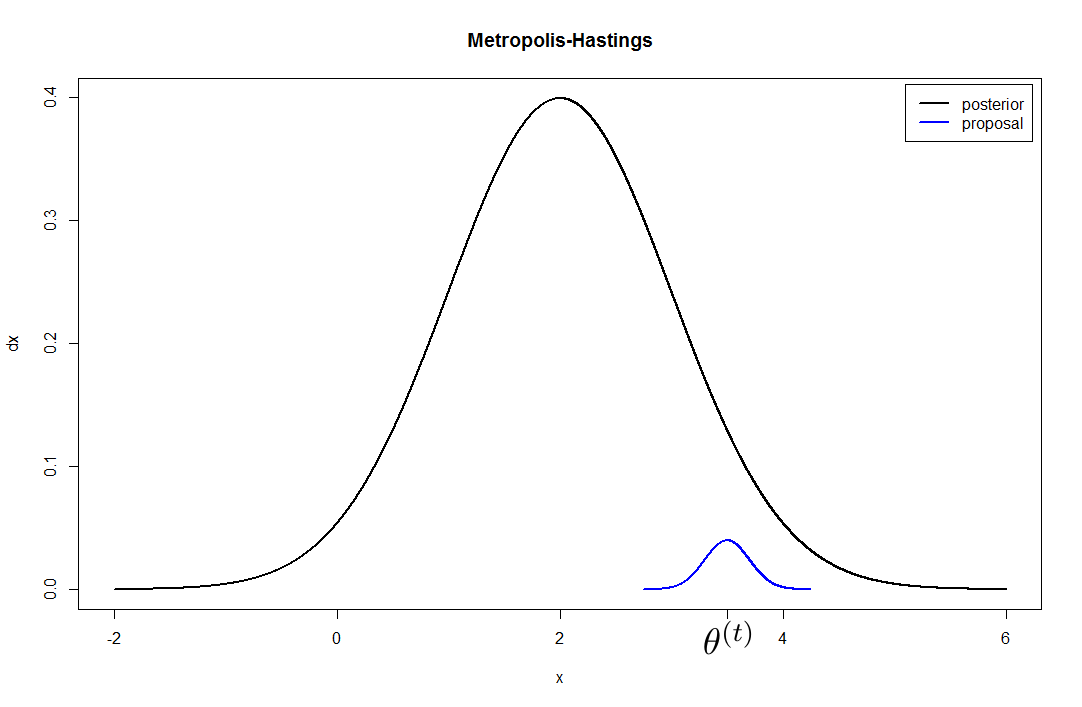
\includegraphics[scale=.38]{MH}
\end{frame}

\begin{frame}
\frametitle{Metropolis--Hastings cont.}
The Metropolis--Hastings algorithm is as follows:\vspace{0.2in}
\begin{enumerate}
\item Given initial values $\boldsymbol\theta^{(0)}$, set $t=1$.
\vspace{0.2cm}
\item Propose $\boldsymbol\theta^\star$ from proposal distribution $J$.
\vspace{0.2cm}
\item Compute acceptance ratio\\ $\hspace{0.2in} r = \frac{f(\boldsymbol\theta^\star | {\bf y})}{f(\boldsymbol\theta^{(t)}|{\bf y})}\frac{J(\boldsymbol\theta^{(t)}|\boldsymbol\theta^\star)}{J(\boldsymbol\theta^\star|\boldsymbol\theta^{(t)})} = \frac{f({\bf y}|\boldsymbol\theta^\star)\pi(\boldsymbol\theta^\star)}{f({\bf y}|\boldsymbol\theta^{(t)})\pi(\boldsymbol\theta^{(t)})}\frac{J(\boldsymbol\theta^{(t)}|\boldsymbol\theta^\star)}{J(\boldsymbol\theta^\star|\boldsymbol\theta^{(t)})}$.
\vspace{0.2cm}
\item Set $\boldsymbol\theta^{(t+1)} = \boldsymbol\theta^\star$ with probability $\min\{1,r\}$, $\boldsymbol\theta^{(t+1)} = \boldsymbol\theta^{(t)}$ otherwise.
\vspace{0.2cm}
\item Increment $t$ by 1 and return to step 2.
\end{enumerate}\vspace{0.2in}
The proposal distribution greatly affects the chain $\{\boldsymbol\theta^{(1)},...,\boldsymbol\theta^{(s)}\}$.  What to do if a nice proposal distribution is hard to find?
\end{frame}

\begin{frame}
\frametitle{Generalized Linear Models (GLM)}
Three major components of a GLM: \vspace{0.2in}
\begin{itemize}
\item Random component:  conditional distribution of $Y_i$ given covariates ${\bf x}_i$, which is a member of the exponential family, i.e.
\[
f(y_i|\mathbf{x}_i) = \exp\left\{\frac{y_i\theta_i - b(\theta_i)}{\phi} + c(y_i,\phi)\right\}
\]
where $\theta_i$ depends on the covariates and parameters.
\vspace{0.2cm}
\item Linear predictor:  $\eta_i = {\bf x}_i^T\boldsymbol\beta$.
\vspace{0.2cm}
\item Link function: $g(\mu_i) = {\bf x}_i^T\boldsymbol\beta$, where $g$ is differentiable and invertible.
\end{itemize}
\end{frame}

\begin{frame}
\frametitle{Bayesian Iteratively Weighted Least Squares (BIWLS)}
\begin{itemize}
\item In the situation where covariates are included, $\boldsymbol\beta$ becomes an unknown parameter of interest.  It can be difficult to find a good proposal distribution for $\boldsymbol\beta$.
\vspace{0.2cm}
\item Placing a normal prior $N({\bf a},{\bf R})$ on $\boldsymbol\beta$, the posterior distribution of $\boldsymbol\beta$ takes form
\[
f(\boldsymbol\beta \mid \mathbf{y}) \propto \exp\left\{ -\frac{1}{2}(\boldsymbol\beta - {\bf a})'{\bf R}^{-1}(\boldsymbol\beta - {\bf a}) + \sum_i \frac{y_i\theta_i - b(\theta_i)}{\phi} \right\}.
\]
\item Approximating this posterior distribution would be a good choice for the proposal distribution.
\end{itemize} 
\end{frame}

\begin{frame}
\frametitle{Bayesian Iterative Re--weighted Least Squares cont.}
\begin{itemize}
\item Consider a transformation of the data and weight matrix:
\[
\widetilde{y}_i(\boldsymbol\beta) = \eta_i + (y_i - \mu_i)g'(\mu_i) \hspace{4mm}\text{and}\hspace{4mm}W_i(\boldsymbol\beta) = \frac{1}{b''(\theta_i)g'(\mu_i)^2}.
\]
\item Carrying out a second order Taylor expansion of the likelihood term
\[
\sum_i \frac{y_i\theta_i - b(\theta_i)}{\phi}
\]
about $\boldsymbol\beta^{(t-1)}$ results in an approximation of $f(\boldsymbol\beta\mid \mathbf{y})$ to be a normal distribution with mean and covariance
\begin{align*}
{\bf m}^{(t)} &= {\bf C}^{(t)}\times\left({\bf R}^{-1}{\bf a} + \frac{1}{\phi}{\bf X}'{\bf W}(\boldsymbol\beta^{(t-1)})\widetilde{{\bf y}}(\boldsymbol\beta^{(t-1)})\right) \\
{\bf C}^{(t)} &= \left({\bf R}^{-1} + \frac{1}{\phi}{\bf X}'{\bf W}(\boldsymbol\beta^{(t-1)}){\bf X}\right)^{-1}.
\end{align*}
\item This means $J = N({\bf m}^{(t)}, {\bf C}^{(t)})$.
\end{itemize}
\end{frame}

\begin{frame}
\frametitle{BIWLS cont.}
Here we summarize Bayesian IRWLS:
\vspace{0.2in}
\begin{enumerate}
\item Given initial values $\boldsymbol\beta^{(0)}$, set $t = 1$.
\vspace{0.2cm}
\item Propose $\boldsymbol\beta^\star$ from proposal distribution $J = N\big{(}{\bf m}^{(t)}, {\bf C}^{(t)}\big{)}$.
\vspace{0.2cm}
\item Compute acceptance ratio $r$.
\vspace{0.2cm}
\item Set $\boldsymbol\beta^{(t+1)} = \boldsymbol\beta^\star$ with probability $\min\{1,r\}$, $\boldsymbol\beta^{(t+1)} = \boldsymbol\beta^{(t)}$ otherwise. 
\item Increment $t$ by 1 and return to step 2.
\end{enumerate}
\vspace{0.2cm}
NOTE: Correction factor in $r$ is necessary! Numerator is density of $\bm\beta^{(t)}$ from $N(\mathbf{m}^\star,\mathbf{C}^\star)$ and denominator is density of $\bm\beta^\star$ from $N\big{(}\mathbf{m}^{(t)},\mathbf{C}^{(t)}\big{)}$.
\end{frame}

\begin{frame}
\frametitle{BIWLS cont.}
~~~~~~~~ 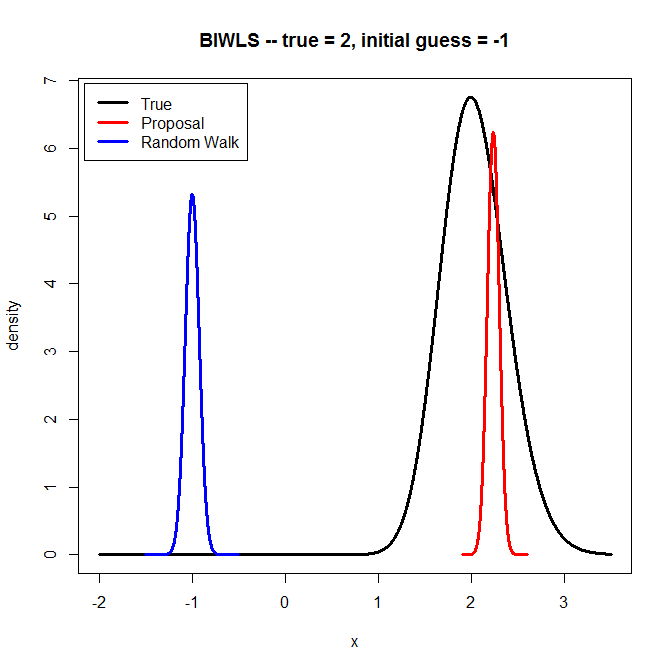
\includegraphics[scale=.35]{BIWLSgraph.png}
\end{frame}

\begin{frame}
\frametitle{Example}
\begin{itemize}
\item Assume the independent data $y_i \sim \text{Bern}(p_i)$, where we impose the logistic link
\[
g(p_i) = \log \dfrac{p_i}{1-p_i} = \mathbf{x}_i'\bm\beta \hspace{5mm}\Longrightarrow\hspace{5mm} p_i = \dfrac{\exp\{\mathbf{x}_i'\bm\beta\}}{1+\exp\{\mathbf{x}_i'\bm\beta\}}.
\]
\item Then the likelihood function is given by
\begin{align*}
f(\mathbf{y}) &= \prod_{i=1}^n p_i^{y_i}(1-p_i)^{1-y_i} \\
&= \exp\left\{\sum_{i=1}^n\left[y_i\log\dfrac{p_i}{1-p_i} + \log (1-p_i)\right]\right\} \\
&= \exp\left\{\sum_{i=1}^n\left[y_i\mathbf{x}_i'\bm\beta - \log\left(1+e^{\mathbf{x}'_i\bm\beta}\right)\right]\right\}.
\end{align*}
\end{itemize}
\end{frame}

\begin{frame}
\frametitle{Example cont.}
\begin{itemize}
\item Therefore the posterior distribution for $\bm\beta$ is given by
\begin{align*}
f(\bm\beta\mid \mathbf{y}) &\propto \exp\Bigg{\{}-\frac{1}{2}(\bm\beta - \mathbf{a})'\mathbf{R}^{-1}(\bm\beta - \mathbf{a}) \\
&\hspace{15mm} + \sum_{i=1}^n\left[y_i\mathbf{x}_i'\bm\beta - \log\left(1+e^{\mathbf{x}'_i\bm\beta}\right)\right]\Bigg{\}}.
\end{align*}
\item Here, $\theta_i = \mathbf{x}_i'\bm\beta, \hspace{1mm}
b(\theta_i) = \log\left(1+e^{\theta_i}\right), \hspace{1mm}\phi=1$.
\end{itemize}
\end{frame}


\begin{frame}
\frametitle{Conclusion}
\begin{itemize}
\item BIWLS improves the acceptance rate in a good way to speed up convergence.
\vspace{0.2cm}
\item Could always accept proposed value, but usually not a good idea.
\vspace{0.2cm}
\item Initial starting point can sometimes affect the BIWLS algorithm.
\vspace{0.2cm}
\item Easily extended to mixed effects models, just affects terms associated with the linear predictor or link function.
\end{itemize}
\end{frame}

\begin{frame}
\frametitle{Bibliography}
\begin{itemize}
\item Gamerman, D.  (1996).  Sampling from the posterior distribution in generalized linear mixed models.  \emph{Statistics and Computing.}
\vspace{0.2cm}
\item Hoff, Peter D. (2010).  A First Course in Bayesian Statistical Methods. \emph{New York: Springer}
\end{itemize}
\end{frame}




\end{document}